% Exemplo de relatório técnico do IC
% Criado por P.J.de Rezende antes do Alvorecer da História.
% Modificado em 97-06-15 e 01-02-26 por J.Stolfi.
% Last edited on 2003-06-07 21:12:18 by stolfi

% modificado em 1o. de outubro de 2008
\documentclass[11pt,twoside]{article}
\usepackage{techrep-ic}

%%% SE USAR INGLÊS, TROQUE AS ATIVAÇÕES DOS DOIS COMANDOS A SEGUIR:
\usepackage[brazil]{babel}
%% \usepackage[english]{babel}

%%% SE USAR CODIFICAÇÃO LATIN1, TROQUE AS ATIVAÇÕES DOS DOIS COMANDOS A
%%% SEGUIR:
%% \usepackage[latin1]{inputenc}
\usepackage[utf8]{inputenc}
\usepackage{graphicx}
\usepackage{url}
\usepackage{multirow}
\usepackage{amsmath}
\usepackage{upgreek}

\bibliographystyle{abbrv}

\begin{document}

%%% PÁGINA DE CAPA %%%%%%%%%%%%%%%%%%%%%%%%%%%%%%%%%%%%%%%%%%%%%%%
% 
% Número do relatório
\TRNumber{???}

% DATA DE PUBLICAÇÃO (PARA A CAPA)
%
\TRYear{12}  % Dois dígitos apenas
\TRMonth{09} % Numérico, 01-12

% LISTA DE AUTORES PARA CAPA (sem afiliações).
\TRAuthor{R. Barboza Jr \and D. C. S. Lucas \and A. S. Ferreira}

% TÍTULO PARA A CAPA (use \\ para forçar quebras de linha).
\TRTitle{Uma Análise Comparativa Entre o Desempenho de Máquinas Virtuais Interpretadas de Sistema e de Processo}

\TRMakeCover

%%%%%%%%%%%%%%%%%%%%%%%%%%%%%%%%%%%%%%%%%%%%%%%%%%%%%%%%%%%%%%%%%%%%%%
% O que segue é apenas uma sugestão - sinta-se à vontade para
% usar seu formato predileto, desde que as margens tenham pelo
% menos 25mm nos quatro lados, e o tamanho do fonte seja pelo menos
% 11pt. Certifique-se também de que o título e lista de autores
% estão reproduzidos na íntegra na página 1, a primeira depois da
% página de capa.
%%%%%%%%%%%%%%%%%%%%%%%%%%%%%%%%%%%%%%%%%%%%%%%%%%%%%%%%%%%%%%%%%%%%%%

%%%%%%%%%%%%%%%%%%%%%%%%%%%%%%%%%%%%%%%%%%%%%%%%%%%%%%%%%%%%%%%%%%%%%%
% Nomes de autores ABREVIADOS e titulo ABREVIADO,
% para cabeçalhos em cada página.
%
\markboth{Barboza, Lucas e Ferreira}{Box}
\pagestyle{myheadings}

%%%%%%%%%%%%%%%%%%%%%%%%%%%%%%%%%%%%%%%%%%%%%%%%%%%%%%%%%%%%%%%%%%%%%%
% TÍTULO e NOMES DOS AUTORES, completos, para a página 1.
% Use "\\" para quebrar linhas, "\and" para separar autores.
%
\title{Uma Análise Comparativa Entre o Desempenho de Máquinas Virtuais Interpretadas de Sistema e de Processo}

\author{
 Roberto Barboza Jr
   \thanks{RA: 035712, rbarboza@gmail.com} \and
 Divino C. S. Lucas
   \thanks{RA: 115121, divcesar@gmail.com} \and
 Anderson Soares Ferreira
   \thanks{RA: 974530, asferreira.ferreira@gmail.com}
}

\date{}

\maketitle

%%%%%%%%%%%%%%%%%%%%%%%%%%%%%%%%%%%%%%%%%%%%%%%%%%%%%%%%%%%%%%%%%%%%%%%%%%%%%%%%%

\begin{abstract} 
Máquinas Virtuais são ferramentas amplamente utilizadas para resolução de 
diversos problemas computacionais e podem ser categorizadas por diversos atributos, 
entre eles escopo de emulação (sistema ou processo) e técnica de emulação 
(interpretação ou tradução). Como forma de ampliar a compreensão do \emph{overhead} 
decorrente da emulação do sistema operacional e dispositivos de \emph{hardware} em uma
máquina virtual de sistema, este trabalho apresenta uma comparação de 
desempenho entre máquinas virtuais interpretadas de sistema e de processo.
Para tanto, conduzimos uma investigação utilizando duas máquinas virtuais distintas. 
A primeira delas, chamada \emph{Bochs}, é uma máquina virtual de sistema que 
emprega interpretação como técnica de emulação, a segunda é uma máquina virtual 
de processo chamada \emph{Box}, desenvolvido a partir da ferramenta anterior 
especificamente para esse estudo.
\end{abstract}






\section{Introdução}
Uma Máquina Virtual (MV) é uma plataforma versátil que pode ser empregada para resolver diversos problemas na área de computação. 
Uma MV pode ser vista como uma camada utilizada para prover a integração entre duas interfaces (possivelmente distintas). 
Esta camada pode ser implementada com emulação em software, virtualização em hardware ou uma composição das duas abordagens.
As interfaces podem ser tanto a \emph{Application Binary Interface} (ABI) em MVs de processo, quanto a \emph{Instruction Set Architecture} (ISA) em MVs de sistema.
Dessa forma, tais ferramentas ocupam uma posição estratégica que pode ser explorada de diversas formas:
\textit{cross-platform emulation} - permitindo que aplicações escritas para uma plataforma sejam executadas em outra; 
\textit{simulação} - simulação do comportamento do hardware durante a execução do programa; \textit{análise} - análise do
perfil de execução das aplicações; \textit{otimização} - aplicar otimizações no código da aplicação utilizando informações
obtidas durante a execução do código.  

Duas abordagens são frequentemente empregadas para implementar a emulação de código em uma máquina virtual: interpretação e tradução.
Uma MV que emprega interpretação utiliza funções para simular o comportamento de cada instrução da aplicação sendo emulada. 
O processo de tradução porém, emprega técnicas da área de compiladores para produzir um código binário nativo (possivelmente otimizado) equivalente àquele da aplicação sendo emulada.
É comum encontrarmos MVs que, visando maximizar o desempenho, empregam estas abordagens em conjunto.

Note que uma MV de sistema emula não apenas as instruções da arquitetura alvo, mas toda uma infraestrutura de hardware
necessária para executar um sistema operacional. Nisto estão inclusos dispositivos como placa de rede, hierarquia de memória,
placa gráfica e etc. Para tarefas como \textit{cross-platform emulation} e perfilamento da execução do código de uma aplicação
em específico, o uso de uma MV de sistema também agrega ao \textit{overhead} de emulação da aplicação o \textit{overhead} de emulação destes 
dispositivos e do sistema operacional. Portanto frequentemente nestes cenários uma máquina virtual de processo é preferível
em relação a uma MV de sistema.

Nesse texto apresentamos uma proposta de avaliação do \textit{overhead} de emulação do sistema operacional e dispositivos de hardware em uma máquina virtual de sistema interpretada em relação a uma máquina virtual de processo interpretada. 

Para tanto, propomos a transformação de uma máquina virtual de sistema em uma máquina virtual de processo. 
Além de uma melhor compreensão do \textit{overhead} de emulação em uma máquina virtual de sistema, este trabalho tem como resultado uma infraestrutura para a realização de experimentos voltados para a área de máquinas virtuais. 

Este texto está organizado da seguinte forma. Na Seção~\ref{sec:objetivos} apresentamos com certo nível de detalhamento nossos objetivos. 
Na Seção~\ref{sec:fundamentacao} apresentamos a fundamentação teórica para a realização do projeto. Na Seção~\ref{sec:bibliografia} apresentamos um levantamento bibliográfico da área de máquinas virtuais a nível de binários. 
A Seção~\ref{sec:infraestrutura} e a Seção~\ref{sec:metodologia} descrevem a infraestrutura e a metodologia proposta para a realização do projeto, respectivamente. 
Por fim a Seção~\ref{sec:conclusao} apresenta a conclusão do trabalho. 
  
  



\section{Fundamentação Teórica} \label{sec:fundamentacao}

\subsection{Máquinas Virtuais}

Uma máquina virtual tem como finalidade implementar as interfaces de um sistema a partir de outro sistema.
Seguindo a taxonomia apresentada por Jim Smith e Nair em \cite{Smith2005}, podemos classificar uma máquina
virtual em de sistema ou de processo dependendo de qual o escopo de emulação é provido:

\begin{itemize}
	\item \textbf{Máquina Virtual de Sistema:} A interface emulada é a nível da \emph{Instruction Set Architecture}. A ISA de
	um computador é composta de duas partes: as instruções de computação de propósito geral (\textit{user-ISA}) e as instruções de 
	controle dos periféricos do sistema (\textit{system-ISA}). Uma máquina virtual de sistema deve, portanto, emular tanto os dispositivos
	de hardware como placas de rede e vídeo quanto as instruções que controlam tais dispositivos. Dessa forma, uma máquina
	virtual de sistema permite a execução de um sistema operacional completo de forma transparente para a aplicação sendo
	emulada. 

	\item \textbf{Máquina Virtual de Processo:} A interface emulada é a nível da \emph{Application Binary Interface}. A ABI  
	define diversos padrões, onde os principais são: um subconjunto da ISA que é visível aos programas de usuário (\textit{user-ISA}) e uma 
	interface para que programas possam se comunicar com o sistema operacional para utilizar os recursos disponíveis no mesmo. 
	Em sistemas operacionais \textit{Unix-like}, esta interface com o sistema operacional é feita através de \emph{system calls} (syscalls). 

	A ABI também define convenções para tipos de dados, \textit{endianness}, alinhamento, chamadas de funções (como devem ser passados 
	os argumentos e o retorno), e o formato utilizado para representar arquivos binários executáveis e bibliotecas dinâmicas.
	No Linux o formato utilizado para representar tais arquivos é o \emph{Executable and Linking Format} (ELF).
\end{itemize}

\subsection{Técnicas de Emulação} \label{emulacao}

Segundo \cite{Smith2005}, a emulação é um processo de implementação das funcionalidades e interfaces de 
um sistema em outro sistema com características diferentes. Por exemplo, para criar uma máquina virtual
que executa um sistema compilado para o x86 em uma arquitetura PowerPC será necessário emular
tanto a interface do x86 (instruções) quanto funcionalidades (ex: \emph{calling convention}) utilizando
instruções disponíveis na arquitetura PowerPC. O processo de emulação é central em uma máquina virtual
e a técnica utilizada para implementá-lo é fundamental para o desempenho do sistema. Entre as técnicas 
frequentemente utilizadas para implementar emulação em uma máquina virtual estão: 

\begin{itemize}
  \item \textbf{Interpretação:} Processo no qual cada instrução do programa original (\emph{guest}) possui 
  uma rotina na plataforma destino (\emph{host}) que implementa a semântica da instrução na arquitetura \emph{guest}. 
  A interpretação envolve a recuperação da instrução original (\emph{fetch}), sua decodificação (\emph{decode}) 
  e finalmente a execução da operação equivalente.
 
  \item \textbf{Tradução de binários:} Neste processo um código nativo na arquitetura destino é gerado 
  dinamicamente (\emph{Just-in-time}) a partir do código original da aplicação e tem como função reproduzir o 
  comportamento do código da aplicação original \cite{Sites1993}. Esta forma de implementação assemelha-se ao
  processo de compilação estático onde um código fonte é decodificado e traduzido para uma linguagem destino.
 
  \item \textbf{Tradução em duas etapas:} Nesta forma de implementação, o sistema utiliza uma combinação de interpretação e tradução com o intuito de
  reduzir o \textit{overhead} de emulação. Regiões de código que são raramente executadas são apenas interpretadas
  (uma vez que o custo de tradução seria maior que o de sempre interpretar a região), enquanto porções de código que são 
  frequentemente executadas são traduzidas, uma vez que a execução do código de forma otimizada amortiza o custo da
  tradução.
\end{itemize}

As implicações do uso de interpretação ou tradução influenciam diretamente o desempenho e a aplicabilidade da 
máquina virtual. Em sistemas interpretados, o desempenho é relativamente baixo, uma vez que cada instrução é 
emulada individualmente por uma função, o que adiciona todo o \textit{overhead} de chamada e retorno de funções. Apesar 
disso, tais sistemas são extremamente portáveis, o que permite sua execução em diversas plataformas com poucas 
ou até mesmo nenhuma alteração em seu código original. Nos sistemas de traduções de binários, existe um custo 
(\emph{overhead}) inicial elevado, visto que o código original precisa ser traduzido antes de sua execução. 
No entanto, uma vez traduzido, o código resultante é executado nativamente, o que garante melhor desempenho. Sistemas
que empregam tradução em duas (ou mais) etapas são ainda mais sofisticados e utilizam técnicas para prever 
regiões de código que serão frequentemente executadas a fim de traduzir e otimizar tais regiões.

\subsection{Técnicas de Otimização para Interpretação}

Na forma mais básica de interpretação há um \textit{loop} principal que busca a instrução original, decodifica-a e chama 
a função responsável pela execução da instrução, retornando ao \textit{loop} principal logo em seguida. No entanto, 
existem diversas técnicas que tornam a interpretação um processo mais eficiente. Algumas delas estão listadas 
a seguir:

\begin{itemize}
 	\item \textbf{Threaded Interpretation:} São adicionadas ao final das funções que emulam cada uma das instruções a 
 	busca pela próxima instrução, sua decodificação e a chamada para a função responsável pela execução da instrução. 
 	Note que isto reduz drasticamente o número de iterações do \textit{loop} principal do interpretador.

 	\item \textbf{Pre Decoding:} As instruções são decodificadas, por exemplo, sempre que uma nova página de código é 
 	carregada do disco, e os campos como \emph{opcode} e operandos são salvos em estruturas de dados padronizadas, o 
 	que torna possível uma implementação mais simples e eficiente dos mecanismos de despacho e interpretação. 
 	
 	\item \textbf{Direct Threaded Interpretation:} Utilizado em conjunto ao \textit{Pre Decoding}. Anota-se junto com
 	as informações de decodificação o endereço da rotina que deve fazer a interpretação de cada instrução, de forma que
 	ao final de cada rotina de interpretação é feito um salto indireto ``diretamente'' para a rotina que interpreta a
 	próxima instrução - evitando a consulta por uma rotina de instrumentação.  

	\item \textbf{DICache:} É uma proposta de utilização de uma cache de decodificação para as instruções interpretadas
	frequentemente. A DICache \cite{dicache} funciona como uma cache convencional e pode ser implementada tanto em software como em 
	hardware. Cada linha da cache contém uma rótulo para identificar a instrução mapeada para aquela linha, os operandos
	da instrução e o endereço da rotina que faz a interpretação dessa instrução.
\end{itemize}

\subsection{Executable and Linking Format}

O \emph{Executable and Linking Format} (ELF) \cite{SCO1997} é o formato de arquivos binários executáveis, 
bibliotecas compartilhadas, códigos objetos, etc. utilizados em ambientes \textit{Unix-like}. Um arquivo ELF
encaixa-se em um dos três tipos:

\begin{itemize}
 	\item \textbf{Relocatable File:} Representa um arquivo objeto que contém dados e código que serão ``linkados" 
 	a outro binário para criar um executável ou objeto compartilhado. Em geral são arquivos utilizados durante
 	o processo de compilação estática.
 
 	\item \textbf{Executable File:} Representa um programa compilado. O programa pode possuir dependências que
 	devem ser resolvidas em tempo de execução ou pode ter ``linkagem" estática, o que significa que todas as bibliotecas
 	necessárias para sua execução já foram resolvidas durante a compilação.
 
 	\item \textbf{Shared Object:} Representa um biblioteca dinâmica que contém código e dados que podem ser 
 	``linkados" a outro objeto compartilhado, criando um terceiro objeto compartilhado, ou pode ser combinado a 
 	um executável pelo \textit{linker} dinâmico e a outros objetos compartilhados para a criação de uma imagem de processo.
\end{itemize}

A organização de um arquivo ELF é composta por um cabeçalho principal (\emph{ELF Header}), seguido por cabeçalhos 
de seção - descrevendo seções de informações (instruções, dados, símbolos) utilizados na ``linkagem" estática - ou cabeçalhos 
de programa - que contém os segmentos da aplicação e as informações necessárias para a criação do processo. 







\section{Levantamento Bibliográfico}  \label{sec:bibliografia}

O Bochs \cite{bochs} é uma máquina virtual de sistema com suporte a emulação 
de diversos processadores da família x86 32 e 64 bits. Ele preza por portabilidade, 
e nesse sentido utiliza interpretação como técnica de emulação. Para reduzir o 
\textit{overhead} de interpretação, o Bochs utiliza técnicas como \emph{pre-decoding}~\cite{Magnusson1994}, 
\emph{threaded-interpretation}~\cite{Klint1981}, e \emph{lazy evaluation}~\cite{Hookway1997}.
O sistema que estamos propondo se diferencia do Bochs por ser voltado à emulação 
de processos e não de sistemas.

O Pin \cite{Luk2005} é uma máquina virtual de processo que emula os ISAs IA-32 e 
x86-64. Ele é uma ferramenta de código fechado e possui versões tanto para Windows 
como para Linux, sendo reconhecido por prover uma rica API para criação de 
ferramentas (Pintools) para análise do comportamento dinâmico de aplicações. O Box 
difere do PIN por ser uma máquina virtual de código aberto e utilizar interpretação 
como técnica de emulação. Em contrapartida, estes dois sistemas tem em comum o 
aspecto de proverem uma interface para instrumentação de binários e serem emuladores 
\emph{same-ISA}~\footnote{Em uma máquina virtual same-ISA as duas interfaces da 
máquina virtual são iguais, possivelmente diferindo apenas em relação a ABI.}.

O HDTrans \cite{Sridhar2006} é uma máquina virtual de processo para a arquitetura 
IA-32. O HDTrans difere do Bochs e do PIN por empregar tradução de binários como 
técnica de emulação. No entanto, o HDTrans abre mão de empregar otimizações no 
código traduzido (o que geralmente é feito para amortizar o \textit{overhead} de tradução) 
em favor da implementação de uma tradução simples e rápida. O Box diferencia-se do 
HDTrans por empregar interpretação de binários.

O Dynamo \cite{Bala2000} é uma máquina virtual de processo para a arquitetura do 
HP PA-8000. Diferentemente do PIN, Bochs e HDTrans, o Dynamo é uma máquina virtual 
cujo objetivo é otimizar a execução do programa sendo emulado. Para tanto, o Dynamo 
emprega uma combinação das técnicas de interpretação e emulação. O sistema 
inicialmente interpreta o código da aplicação sendo emulada. Uma vez que uma região 
é declarada como quente~\footnote{Uma região de código é quente quando ela é 
frequentemente executada.}, o Dynamo aplica otimizações nesta região e salva o 
código otimizado em uma cache de traduções. Subsequentes invocações do trecho de 
código original serão emuladas utilizando o código traduzido. O Box diferencia-se 
do Dynamo por não ter o foco na otimização de binários mas sim em ser um sistema 
que disponibilize uma interface simples para instrumentação de binários.

O IA-32 EL \cite{Baraz2003} é uma máquina virtual de processos com o objetivo de 
suportar a execução de aplicações IA-32 em processadores da família IA-64. De forma 
similar ao Dynamo, o IA-32 EL emprega uma abordagem de emulação em duas etapas, 
porém as duas etapas realizam tradução de código. Inicialmente o IA-32 EL efetua a 
tradução de código em uma granularidade de bloco básico. Durante essa tradução, 
código de instrumentação é inserido para detectar blocos básicos quentes. Quando um 
número mínimo de blocos básicos é identificado, o sistema forma uma região de código 
envolvendo esses blocos básicos, os otimiza e posteriormente salva em uma cache de 
traduções. Execuções subsequentes desses blocos básicos usam a tradução otimizada. 
O Box diferencia-se do IA-32 EL por não fazer tradução de binários.

O StarDBT \cite{Wang2007} é uma máquina virtual de pesquisa capaz de fazer traduções de 
aplicações compiladas para x86 32/64 bits para execução em hardware x86 32 bits. De 
forma similar ao IA-32 EL e ao Dynamo, o StarDBT é um tradutor em duas fases. Regiões 
de código que são infrequentemente executadas são traduzidas utilizando um tradutor 
simples e rápido, enquanto regiões de código que são frequentemente executadas são 
traduzidas empregando otimizações de código e posteriormente persistidas em uma cache 
de traduções. O Box diferencia-se do StarDBT por ser capaz de traduzir apenas binários 
de 32 bits, compilados para Linux e não empregar tradução de binários.

% Acho que seria interessante colocarmos alguns papers que investigaram sobre
% o overhead de emulação em máquinas virtuais, especificamente sobre a emulação
% de sistemas operacionais em relação a processos. Será que achamos? Será que tem? 




\section{Infraestrutura de Pesquisa} \label{sec:infraestrutura}

Nessa seção descrevemos em detalhes as principais ferramentas que
utilizamos para desenvolver esse projeto. Inicialmente apresentamos
os detalhes mais relevantes da máquina virtual de sistema Bochs, 
posteriormente apresentamos a máquina virtual de processos Box, que
foi desenvolvida a partir do Bochs especificamente para este projeto.
As duas últimas subseções desta seção descrevem os benchmarks 
utilizados para realizar os experimentos e as bibliotecas de runtime
utilizadas por estes benchmarks.

\subsection{Bochs}

O Bochs é uma máquina virtual de sistema que utiliza interpretação como
técnica de emulação das instruções, veja Figura~\ref{fig:bochs}. Sendo 
uma máquina virtual de sistema o Bochs necessita fazer a emulação de 
diversos componentes de sistema, tais como: placa de vídeo, rede, som,
dispositivos de disco, cdrom, mouse e teclado além de dispositivos de
componentes internos da arquitetura como cache de instruções, segmentação,
TLB, etc.

O Bochs utiliza alguns mecanismos para acelerar a interpretação das 
aplicações, como por exemplo trace cache e threaded-interpretation.
A Figura~\ref{fig:bochs_loop} mostra o laço principal de interpretação 
de instruções do Bochs, na sua versão mais básica. O corpo do laço
é composto de seis partes, detalhadas a seguir:

\begin{figure}[!h]
  	\begin{center}
    	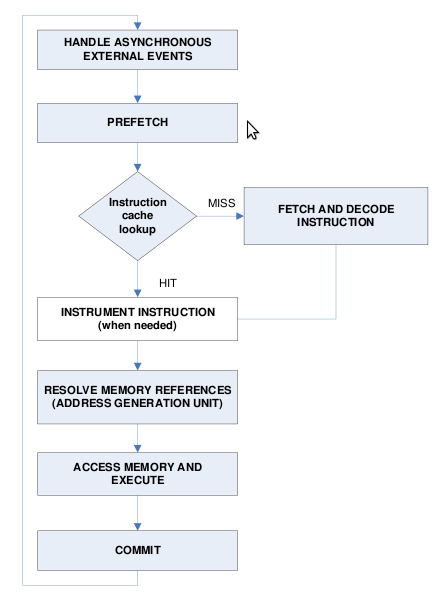
\includegraphics[scale=0.5]{figures/bochs_loop.png}
	\end{center}
	\caption{Laço principal de interpretação de instruções do Bochs}
	\label{fig:bochs_loop}
\end{figure}

\begin{itemize}
	\item \textbf{Events:} Nesse estágio ocorre a verificação se ocorreu alguma
	interrupção ou ``trap'' durante a interpretação da instrução
	anterior. Note que o Bochs possui suporte a execução de traços e
	threaded-interpretation. Essa verificação é feita apenas quando
	a execução volta ao laço principal de interpretação.

	\item \textbf{Prefetch:} Nesse estágio ocorre a verificação de permissões 
	de acesso a página de código, validação de limites de segmento e 
	o cálculo do endereço ``host'' da próxima instrução a ser emulada.

	\item \textbf{Decode:} Nesse estágio ocorre a busca e decodificação da
	instrução a ser emulada. O Bochs possui uma cache interna das 
	instruções mais recentemente decodificadas, se a instrução a
	ser interpretada estiver na cache as informações são reutilizadas
	caso contrário a instrução é decodificada.

	\item \textbf{Instrumentation:} Nesse estágio o Bochs verifica se a
	instrução a ser interpretada é alvo de alguma rotina de 
	instrumentação. Em caso afirmativo a rotina de instrumentação é
	invocada antes da interpretação da instrução.

	\item \textbf{Memory Addresses:} Nesse estágio endereços de memória
	utilizados pela instrução a ser interpretada são resolvidos.
	Em outras palavras, este passo é o responsável por tratar as
	várias formas de endereçamento presentes na família x86.

	\item \textbf{Execution:} Nesse estágio ocorre de fato a interpretação 
	da instrução. Durante a decodificação da instrução, a rotina
	que deve efetuar a interpretação é anotada como meta-informação
	da instrução, este estágio utiliza essa informação para fazer
	uma chamada indireta para essa rotina.

	\item \textbf{Commit:} Esse estágio faz a consolidação da execução da
	instrução, isto é, atualiza o registrador EIP.

\end{itemize}


\subsection{Box}

Nesta seção descrevemos os principais componentes da máquina virtual 
de processo Box e os maiores desafios que enfrentamos durante o seu 
desenvolvimento.

Embora estas duas máquinas virtuais (Bochs e Box) sejam similares 
conceitualmente (emulação de uma interface em cima de outra) elas
possuem uma arquitetura drasticamente diferente. Por exemplo, 
uma vez que o Bochs faz a execução de um sistema operacional ele
não precisa se preocupar com detalhes de criação de processos ou
chamadas de sistema, porém uma máquina de processos geralmente
precisa. Da mesma forma, uma máquina virtual de processo não precisa
emular o conceito de discos rigidos, placas de vídeo, rede, etc. uma
vez que esses recursos não são diretamente visiveis ao processo.


\subsubsection{Componentes Removidos}

Todos os componentes de hardware que não são diretamente acessados
pelos processos foram removidos, isso enclui placa de vídeo, placa de
rede, placa de som, mouse, teclado, cdrom, disco rigido, diskete, portas
USB, PCI, COM, etc.

Além dos componentes de hardware, também ouve grande modificação na 
forma como os acessos a memória do programa guest são feitos. O Bochs 
faz a simulação de caches de instrução, dados, e translation lookasside 
buffer (TLB), no nenhum desses componentes foi mantido no Box.

\subsubsection{Carregador}

A implementação atual do Box não conta con nenhum auxilio do kernel do
sistema operacional para montar o espaço de endereçamento da aplicação
sendo emulada. Enquanto isso foi escolhido para permitir a emulação de
todo o processo de carregamento e execução da aplicação, isso trouxe 
uma serie de complicações para o desenvolvimento do projeto.

Não contar com o suporte do kernel significa que teremos que implementar
no projeto toda a infraestrutura de código responsável por fazer o 
carregamento e ligação do executável principal e bibliotecas compartilhadas,
bem como criar o espaço de endereçamento inicial da aplicação.

Durante as etapas iniciais de desenvolvimento do projeto, o objetivo era
o desenvolvimento de um carregador suficientemente poderoso para suportar
a execução de aplicativos compilados com linkagem dinâmica utilizando a
biblioteca de runtime Glibc~\cite{glibc}. O desenvolvimento deste carregador
avançou até o ponto de ser possivel executar pequenas aplicações com linkagem
dinâmica, mas sem o uso da Glibc. Nesse ponto percebemos que o desenvolvimento
do carregador da forma inicialmente proposta gastaria mais tempo que o 
disponível para a realização do projeto, e dessa forma, foi decidido que
a primeira versão do Box seria capaz de executar apenas aplicações 
estaticamente compiladas utilizando a biblioteca de runtime $\upmu$ClibC.

A principal tarefa do carregador atualmente implementado no Box é 
encontrar o executável principal da aplicação, fazer o seu parcing e
montar o espaço de endereçamento onde a aplicação executará. A primeira
tarefa é simples, uma vez que o usuário passa o endereço completo da
aplicação como parâmetro para o Box. O executável deve estar códificado
no formato ELF-32~\cite{elf} e não fazer uso de linkagem dinâmica. A 
segunda tarefa do carregador é fazer o parsing do executável e encontrar
quais segmentos (geralmente dois segmentos, um de texto e outro de dados) 
de código devem ser carregados na memória. Uma vez que esses segmentos 
tenham sido encontrados o carregador começa a montar o espaço de 
endereçamento do processo. O espaço de endereçamento é montado seguindo
a mesma estrutura que seria utilizada pelo carregador nativo do Linux e
é exemplificado na Figura~\ref{fig:esp_end} para os casos com linkagem
dinâmica e estática.

Outra tarefa desempenhada pelo kernel/carregador nativo do SO e que
precisou ser implementada no Box foi a estrutura inicial da pilha de
execução da aplicação. Além dos parâmetros e variáveis de ambiente a
pilha inicial contém informações que o kernel passa para o carregador
nativo do sistema, estas informações podem/são usadas tanto pelo
carregador quanto pela biblioteca de runtime utilizada. Essas informações,
são passadas na forma de um vetor e contém dados como por exemplo, 
tamanho de página no sistema, endereço onde o cabeçalho ELF do 
programa foi carregado, entre outras coisas. A Figura~\ref{fig:stack_ini}
mostra o formato inicial da pilha de execução de um programa.


\subsubsection{Emulação de Syscalls}

\subsubsection{Emulação da Memória}

\subsection{Mibench}

\subsection{$\upmu$ClibC}





\section{Resultados} \label{sec:resultados}

\subsection{Metodologia}

\subsection{Overhead de Emulação de Sistema}

Comparação com o Bochs.

\subsection{Otimizando a Interpretação}

Gráficos mostrando o tempo de execução do Box com DICache, Threaded Interpretation
e ambas as técnicas habilitadas.

\subsection{Caracterizando o Overhead do Sistema}

Gráfico, por exemplo na forma de pizza, mostrando quais são os pontos onde o Box
gasta a maior parte do tempo durante a emulação.







\section{Conclusão}  \label{sec:conclusao}




\newpage
\bibliography{box}




\end{document}
